% !TEX root = ../Coherence2.tex

\section{Hypergraph polytopes} 
\label{s:hypergraph}

In this section, we recall the definition of hypergraph polytopes. 
We refer to \cite{DP-HP,COI} for more details. 

%%%%%%%%%%%%%%%%%%%%%%%%%%%%%%%%%%%%%%%%%%%

\subsection{Hypergraphs}
A \defn{hypergraph} is given by a finite set $H$ of \defn{vertices} and a subset of \defn{hyperedges} $\hyper{H}\inc {\cal P}(H)\setminus\emptyset$ such that $\Union \hyper{H}=H$. 
We say that $\hyper{H}$ is \defn{ordered} if $H$ is equipped with a total order.
We always assume that $\hyper{H}$ is \defn{atomic}, that is $\set{x}\in \hyper{H}$, for all $x\in H$. 
A hyperedge of cardinality 2 is called an \defn{edge}.  
For $X\inc H$, the \defn{plain restriction} of $\hyper{H}$ to $X$ is the set 
$\hyper{H}_X \eqdef   \setc{Z\in \hyper{H}}{\; Z\inc X}$.

We say that $\hyper{H}$ is \defn{connected} if there is no non-trivial partition $H=X_1\union X_2$ such that $\hyper{H}=\hyper{H}_{X_1}\union \hyper{H}_{X_2}$. 
For each hypergraph, there exists a partition $H=X_1\union\ldots\union X_m$ such that each $\hyper{H}_{X_i}$ is connected and $\hyper{H}=\Union(\hyper{H}_{X_i})$.  
The $\hyper{H}_{X_i}$'s are called the \defn{connected components} of $\hyper{H}$.
We say that a non-empty subset $X\inc H$ of vertices is \defn{connected} (resp. a \defn{connected component}) whenever $\hyper{H}_X$ is connected (resp. a connected component of $\hyper{H}$).  Thus our uses of ``connected'' in the sequel will always carry the non-emptyness information.
We denote by $\restrH{H}{X}\eqdef  \hyper{H}_{H\setminus X}$ the plain restriction of $\hyper{H}$ to $H \setminus X$.
The \defn{saturation} of $\hyper{H}$ is the hypergraph
$\Sat(\hyper{H})\eqdef  \setc{X}{\emptyset\incs X\inc H\;\mbox{and}\;\hyper{H}_X\;\mbox{is connected}}$.
A hypergraph is called \defn{saturated} when $\hyper{H}=\Sat(\hyper{H})$.  
The \defn{reconnected restriction} of $\hyper{H}$ to $X$ is the set $$\recrestr{\hyper{H}}{X}\eqdef  \setc{Z\cap X}{Z\in \Sat(\hyper{H}), Z\cap X\neq\emptyset}.$$

\begin{rem}
    Atomic and saturated hypergraphs are called \defn{building sets} in the  literature on nestohedra, see for example \cite{P09,FS05}.
\end{rem}

For $X\inc H$, we will express the fact that $\setc{H_i}{i\in I}$ is the set of connected components of $\restrH{H}{X}$ by the notation $\hyper{H},X  \leadsto  \setc{H_i}{i\in I}$.
If $\hyper{H}$ is ordered, we order the connected components by \defn{increasing order} of their maximal vertices, \textit{i.e.}, $\setc{H_i}{i\in I}=\{H_{i_1}<\cdots < H_{i_n}\}$, and we write $\hyper{H},X  \leadsto H_{i_1},\ldots,H_{i_n}$.
In the specific situation where $x,y,z\in H$ and $\hyper{H},\set{x}\leadsto \setc{H_i}{i\in I}$, we shall write
$$\begin{array}{ll}
\xyz{x}{\hyper{H}}{\set{y,z}} & \mathrm{if}\; y,z\in H_i\; \mbox{for some}\; i \in I\\
\xyz{x}{\hyper{H}}{\set{y},\set{z}} & \mbox{otherwise}.
\end{array}$$
In the second case, we will say that $x$ \defn{disconnects} $y$ and $z$ in $\hyper{H}$. 
The reconnected restriction allows one to characterize the preceding two situations as follows.

\begin{lemma} 
\label{xyz-reconnected} 
We have
$$\begin{array}{lll}
\xyz{x}{\hyper{H}}{\set{y,z}} & \mathrm{iff} & \recrestr{\hyper{H}}{\set{x,y,z}},\set{x}\leadsto\set{y,z} \\
\xyz{x}{\hyper{H}}{\set{y},\set{z}} & \mathrm{iff} & \recrestr{\hyper{H}}{\set{x,y,z}},\set{x}\leadsto \set{y},\set{z}.
\end{array}$$
\end{lemma}

\begin{proof} 
    Let $\hyper{H},\set{x}\leadsto \set{H_1,\ldots,H_n}$. 
    Suppose that $\xyz{x}{\hyper{H}}{\set{y,z}}$. 
    Then there exists $i$ such that~$\set{y,z}\inc H_i$, and hence $\set{y,z}\inc H_i\cap\set{x,y,z}$, and in fact $\set{y,z} = H_i\cap\set{x,y,z}$ since~$x\not\in H_i$. 
    Thus $\recrestr{\hyper{H}}{\set{x,y,z}},\set{x}\leadsto\set{y,z}$ holds by definition of reconnected restriction.
    If to the contrary we have $\xyz{x}{\hyper{H}}{\set{y},\set{z}}$, then there exists $i\neq j$ such that $y\in H_i$ and~$z\in H_j$. 
    We then derive likewise that $H_i\cap\set{x,y,z}=\set{y}$ and $H_j\cap\set{x,y,z}=\set{z}$ from which $ \recrestr{\hyper{H}}{\set{x,y,z}},\set{x}\leadsto \set{y},\set{z}$ follows.
    The reverse implications are immediate.
\end{proof}

%%%%%%%%%%%%%%%%%%%%%%%%%%%%%%%%%%%%%%%%%%%%%%%%%%%%%%%

\subsection{Constructs}
A {connected} hypergraph $\hyper{H}$ gives rise to a set of \defn{constructs}, which are defined inductively as follows.
 
\begin{definition} 
\label{inductive-construct}
%as follows.
Let $\hyper{H}$ be a connected hypergraph and $Y$ be a non-empty subset of $H$.
\begin{enumerate}
\item  If $Y = H$, then the one-node tree $H$ decorated with $H$ is a construct of $\hyper{H}$.
\item If $\hyper{H},Y  \leadsto \{H_1,\ldots,H_n\}$, and if $T_1,\ldots,T_n$ are constructs of $\hyper{H}_1,\ldots,\hyper{H}_n$, respectively, then the
non-planar tree $Y(T_1,\ldots,T_n)$ whose root is decorated by $Y$, with $n$ outgoing edges on which the respective $T_i\,$'s are grafted is a construct.  
\end{enumerate}
In the notation $Y(T_1,\ldots,T_n)$, no order is intended on  $T_1,\ldots,T_n$.
However, when $\hyper{H}$ is ordered, the trees $T_1,\ldots,T_n$ are listed according to the order given by $\hyper{H},Y  \leadsto H_1,\ldots,H_n$, making constructs planar.
When $Y={z}$ is a singleton, we freely write $z$ in place of $\set{z}$.
A \defn{construction} is a construct all of whose nodes are  decorated with singletons. 
\end{definition}


Since all decorations in a construct are disjoint, we freely identify nodes with subsets of~$H$. 
We use the notation $\occ{T}{X}$ to denote the  subtree of $T$ rooted at $X$, defined only if $X$ is indeed a decoration of a node of $T$. 
If $S$ is a subtree of $T$, we denote by $\supp(S)$ the union of the decorations of the nodes of $S$.

\begin{rem} \label{subconstruct-restriction}
The intention behind this presentation is algorithmic: a construct is built by picking and removing a non-empty subset $Y$ of $H$, then branching to the connected components of $\restrH{H}{Y}$ and continuing inductively in all the branches.
It follows readily from the definition that $\occ{T}{X}$ is a construct of $\hyper{H}_{\supp(\occ{T}{X})}$.
\end{rem}

\begin{rem}
    The notion of construct is equivalent to the notion of nested set \cite{P09}, and to the notion of tubing in the case where $\hyper{H}$ is a graph~\cite{CD-CCGA}.  
    We refer to \cite[Sec.~3.1]{COI} for details.
\end{rem}

%Here we content ourselves with a sketchy description of the
%dictionary (for the readers familiar with nested sets).
%Given a construct $T$, take the set $\setc{\supp(\occ{T}{X})}{X\:\textrm{is a node of}\: T}$. Conversely, read a construct from a nested set $\mathbb{T}$ as follows: for each  $Z\in\mathbb{T}$, consider the elements $Z_1,\ldots, Z_n\in\mathbb{T}$ that are maximal among all elements of $\mathbb{T}$ that are strictly included in $Z$, then $Z\setminus\bigcup(Z_1\cup \ldots \cup Z_n)$ will decorate a node of the corresponding construct. 
%The subface relation formulated in terms of nested sets is just the inclusion of nested sets.

If $X,Y$ are two nodes of a construct $S$ of $\hyper{H}$, $X$ being the father of $Y$, we can define a new construct $T$ by contracting the edge between $X$ and $Y$, and labeling the resulting vertex of~$T$ by the union of the labels of $X$ and $Y$. 
Formally, if $X$ is a node of $S$ such that $\occ{S}{X}=X(Y(S_1,\ldots,S_m),S_{m+1},\ldots S_n)$, then  $T$ is obtained by replacing in $S$ the  subtree rooted at $X$ with $(X\cup Y)(S_1,\ldots,S_n)$.  
We say that $T$ \defn{covers} $S$ and use the notation $S\prec T$.


\begin{definition} 
  \label{subface-relation}
    We denote $({\cal A}(\hyper{H}),\prec^*)$ the poset of constructs of a connected hypergraph~$\hyper{H}$ obtained as the reflexive and transitive closure of the  covering relation $\prec$.    
\end{definition}
    
We shall need the following lemma.
\begin{lemma} 
  \label{partial-construct}
Let $\hyper{H}$ be a connected hypergraph. 
If $\hyper{H},X\leadsto \{H_1,\ldots,H_n\}$ and if constructs $T_i$ of~$\hyper{H}_i$ are given for all $i\in I\subseteq \set{1,\ldots,n}$, then $X(\setc{T_i}{i\in I})$ is a construct of $\recrestr{\hyper{H}}{(H\setminus\cup\setc{H_j}{j\not\in I})}$.
\end{lemma}
\begin{proof} This is an immediate consequence of the following two observations: we have
$$\recrestr{\hyper{H}}{(H\setminus\cup\setc{H_j}{j\not\in I})},X\leadsto \setc{H_i}{i\in I}\;\; \mbox{and}\;\; (\recrestr{\hyper{H}}{(H\setminus\cup\setc{H_j}{j\not\in I})})_{H_i}=\hyper{H}_{H_i}=\hyper{H}_i.$$
\end{proof}

%%%%%%%%%%%%%%%%%%%%%%%%%%%%%%%%%%%%%%%%%%%%%%

\subsection{Hypergraph polytopes}
\label{ss:hypergraph-polytopes}

We are now ready to define hypergraph polytopes, a.k.a nestohedra.

\begin{definition}
    A \defn{hypergraph polytope} is a polytope whose face lattice is isomorphic to the poset of constructs of some connected hypergraph $\hyper{H}$.
\end{definition}

Do\v sen and Petri\'c gave polytopal realizations of hypergraph polytopes in ~\cite{DP-HP}.
The idea is that the connected subsets of $\hyper{H}$ specify the faces of a fixed $(|H|-1)$-dimensional simplex that are to be truncated.
% according to the constructs of $\hyper{H}$.

Let us introduce a few families of hypergraph polytopes that will be studied in \cref{ss:examples}.
When $\hyper{H}$ is a graph, hypergraph polytopes are known as \emph{graph-associahedra} \cite{CD-CCGA}.

\subsubsection{Simplices}
The $n$-dimensional \defn{simplex} is the realization of the hypergraph 
$$\mathbb{S}_n\eqdef  \{\{1\},\{2\},\ldots,\{n+1\},\{1,\ldots,n+1\}\}.$$

\subsubsection{Cubes}
The $n$-dimensional \defn{cube} is the realization of the hypergraph
$$\mathbb{C}_n\eqdef  
\{\{1\},\{2\},\ldots,\{n+1\}\}\cup\{\{j \ | \ 1 \leq j \leq i \} \ | \ 1 \leq i \leq n+1\}.$$
Note that these two families of hypergraph polytopes are defined by genuine hypergraphs, contrary to the following families of graph-associahedra.

\subsubsection{Associahedra}
The $n$-dimensional \defn{associahedron} is the realization of the graph 
$$\mathbb{K}_n\eqdef  \{\{1\},\{2\},\ldots,\{n+1\},\{1,2\},\ldots,\{n,n+1\}\}.$$
In other words, it is the graph-associahedron for the linear graph with $n+1$ vertices.

\subsubsection{Permutahedra}
The $n$-dimensional \defn{permutahedron} is the realization of the graph 
$$\mathbb{P}_n\eqdef  \{\{1\},\{2\},\ldots,\{n+1\}\} \cup \{\{i,j\} \ | \ 1 \leq i \neq j \leq n+1 \}.$$
In other words, it is the graph-associahedron for the complete graph on $n+1$ vertices.

Note that the definition of $\hyper{S}_n$ and $\hyper{P}_n$ does not depend on any order on the vertices, while the definition of $\hyper{C}_n$ and $\hyper{K}_n$ involves the total order on~$\set{1\ldots,n+1}$. 

\begin{rem}
  In the above descriptions, we can replace $\set{1,\ldots,n+1}$ by any finite set $X=\set{x_1,\ldots,x_{n+1}}$  (resp. any finite linear order $X=x_1<\cdots<x_{n+1}$)  and define $\hyper{S}^X$ and $\hyper{P}^X$ (resp. $\hyper{C}^X$, $\hyper{K}^X$) accordingly.
\end{rem}


\subsubsection{Operahedra}
To every  planar tree $\calT$ with $n+2$ vertices, one can associate its $n$-dimensional \defn{operahedron}, whose faces are in bijection with the nestings of $\calT$ \cite{laplante-anfossiDiagonalOperahedra2022a,CLA1}, which in turn
are in bijection with the tubings of the \defn{line graph} $\mathbb{L}(\calT)$ of $\calT$.
The vertices of $\mathbb{L}(\calT)$ are the edges of ${\cal T}\!$, and two vertices are connected whenever as edges of ${\cal T}$ they share a common vertex, see \cref{fig:line-graph}.
In other words, an $n$-dimensional operahedron is the graph-associahedron of a clawfree block graph with $n+1$ vertices.

\begin{figure}[h!]
  \begin{center}
    \begin{tabular}{ccc}
    \resizebox{2cm}{!}{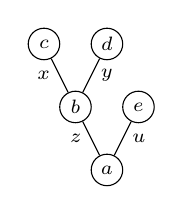
\begin{tikzpicture}[scale=0.8]
        % set up the nodes
        \node (E)[circle,draw=black,minimum size=4mm,inner sep=0.1mm] at (0,0) {\scriptsize $a$};
        \node (F) [circle,draw=black,minimum size=4mm,inner sep=0.1mm] at (-0.5,1) { \scriptsize $b$};
        \node (A) [circle,draw=black,minimum size=4mm,inner sep=0.1mm] at (0.5,1) {\scriptsize $e$};
        \node (Asubt) [circle,draw=black,minimum size=4mm,inner sep=0.1mm] at (-1,2) {\scriptsize  $c$};
        \node (P) [circle,draw=black,minimum size=4mm,inner sep=0.1mm] at (0,2) {\scriptsize $d$};
        % draw arrows and text between them
        \draw[-] (E)--(F) node  [midway,left] {\scriptsize $z$};
        \draw[-] (E)--(A) node  [midway,right] {\scriptsize $u$};
     \draw[-] (F)--(Asubt) node [midway,left] {\scriptsize $x$};
     \draw[-] (F)--(P) node [midway,right] {\scriptsize $y$};
       \end{tikzpicture}}
    
    &&
    \resizebox{2cm}{!}{
    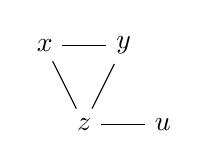
\begin{tikzpicture}
        % set up the nodes
        \node (Z)[] at (-0.5,0) {$z$};
        \node (U)[]  at (0.5,0) {$u$};
        \node (X)[]  at (-1,1) {$x$};
        \node (Y)[]  at (0,1) {$y$};
        % draw arrows and text between them
        \draw[-] (Z)--(U) node  {};
     \draw[-] (Z)--(X) node  {};
     \draw[-] (Z)--(Y) node {};
     \draw[-] (X)--(Y) node {};
       \end{tikzpicture}}
    \end{tabular}
    \end{center}
    \caption{A planar tree with $5$ vertices (left) and its line graph (right).}
    \label{fig:line-graph}
\end{figure}

Many more examples are to be found in~\cite{DP-HP,COI,CDOO}, as well as in the abundant literature on nestohedra.



